\section{Results}
\label{sec:results}

Cosmological constraints

\begin{figure}
	\begin{center}
		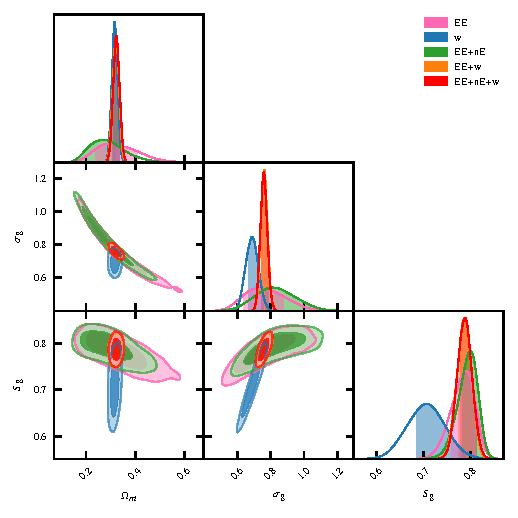
\includegraphics[width=\columnwidth]{Parameter_Plots/omegam_sigma8_s8_blind_A}
		\caption{Constraints on flat $\Lambda$CDM blind A}
		\label{fig:cosmology-params}
	\end{center}
\end{figure}

\begin{figure}
	\begin{center}
		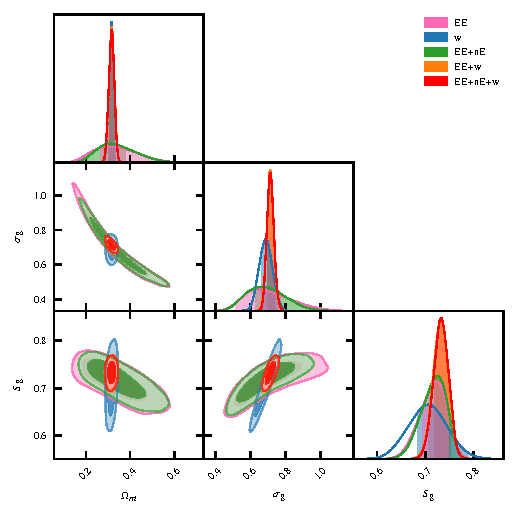
\includegraphics[width=\columnwidth]{Parameter_Plots/omegam_sigma8_s8_blind_B}
		\caption{Constraints on flat $\Lambda$CDM blind B}
		\label{fig:cosmology-params}
	\end{center}
\end{figure}

\begin{figure}
	\begin{center}
		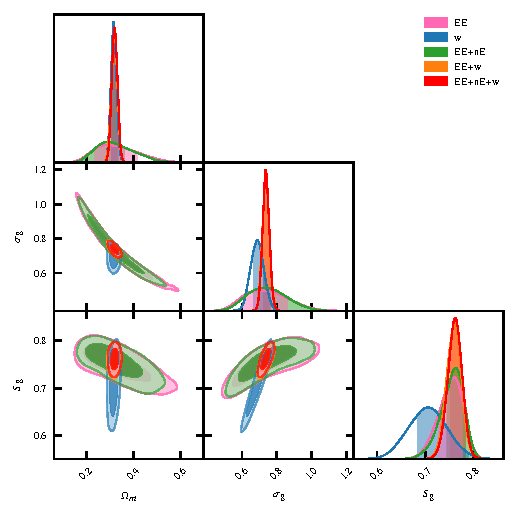
\includegraphics[width=\columnwidth]{Parameter_Plots/omegam_sigma8_s8_blind_C}
		\caption{Constraints on flat $\Lambda$CDM blind C}
		\label{fig:cosmology-params}
	\end{center}
\end{figure}


\begin{figure}
	\begin{center}
		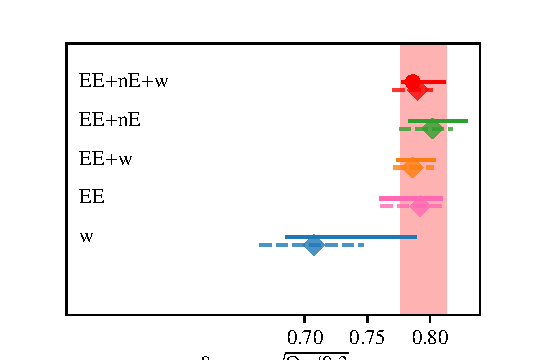
\includegraphics[width=\columnwidth]{Parameter_Plots/S8_comparison_blindA}
		\caption{Constraints on $S_{8}$ blind A}
		\label{fig:cosmology-params}
	\end{center}
\end{figure}

\begin{figure}
	\begin{center}
		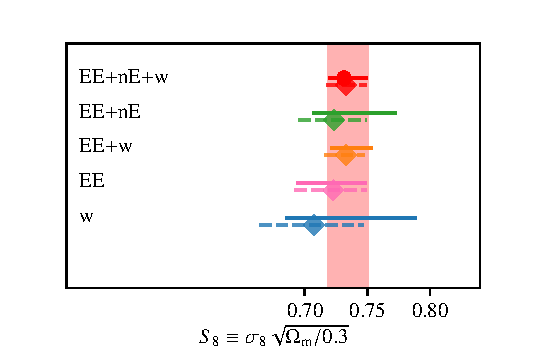
\includegraphics[width=\columnwidth]{Parameter_Plots/S8_comparison_blindB}
		\caption{Constraints on $S_{8}$ blind B}
		\label{fig:cosmology-params}
	\end{center}
\end{figure}

\begin{figure}
	\begin{center}
		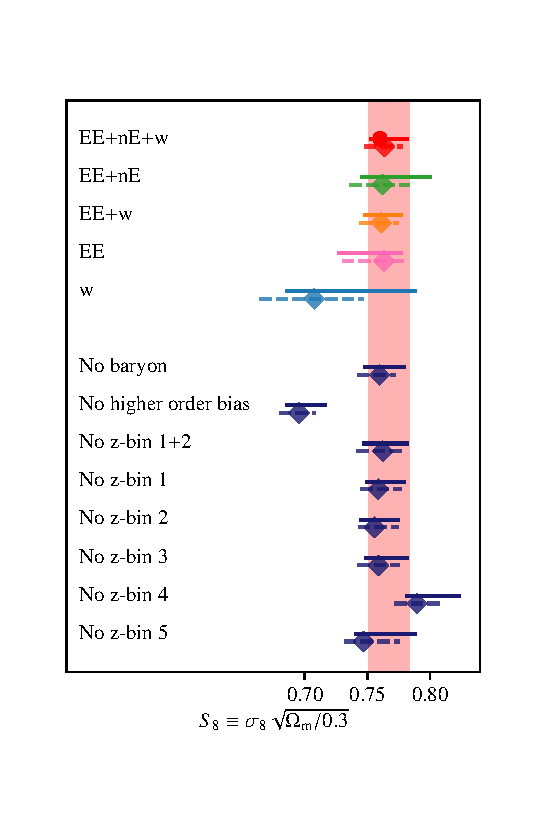
\includegraphics[width=\columnwidth]{Parameter_Plots/S8_comparison_blindC}
		\caption{Constraints on $S_{8}$ blind C}
		\label{fig:cosmology-params}
	\end{center}
\end{figure}

\begin{figure*}
	\begin{center}
		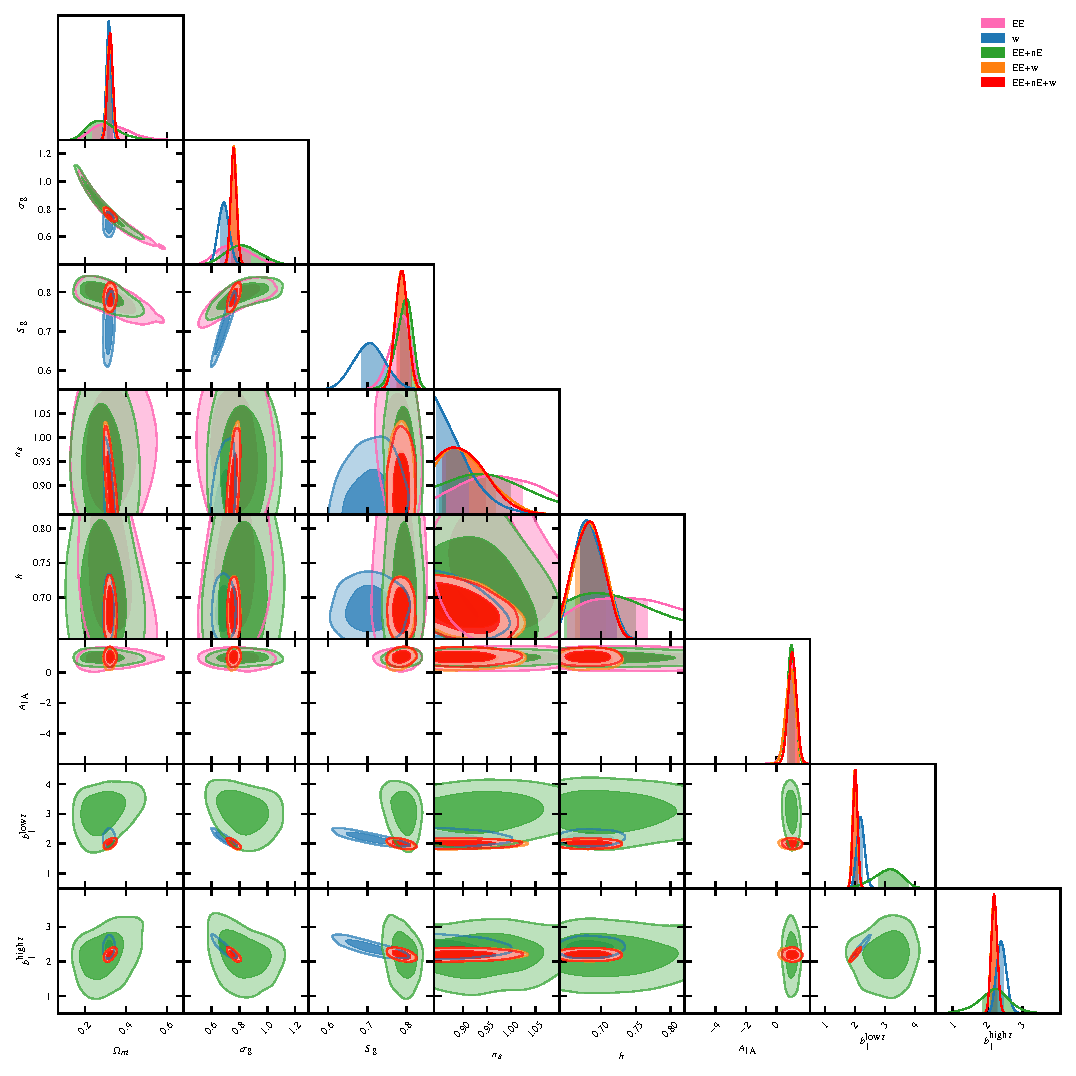
\includegraphics[width=\textwidth]{Parameter_Plots/omegam_sigma8_s8_ns_h_a_ia_b1l_b1h_blind_A}
		\caption{Constraints blind A}
		\label{fig:cosmology-params}
	\end{center}
\end{figure*}

\begin{figure*}
	\begin{center}
		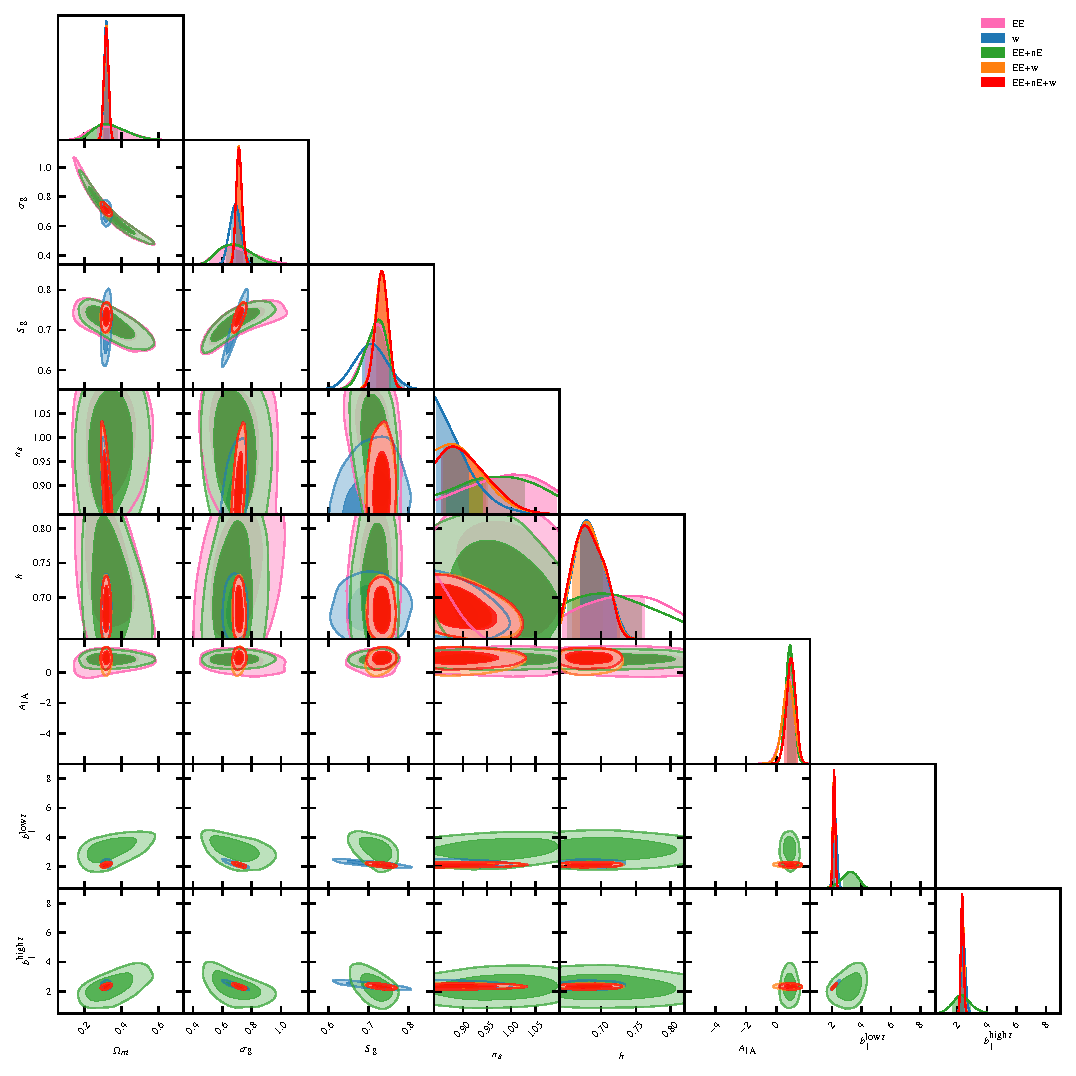
\includegraphics[width=\textwidth]{Parameter_Plots/omegam_sigma8_s8_ns_h_a_ia_b1l_b1h_blind_B}
		\caption{Constraints blind B}
		\label{fig:cosmology-params}
	\end{center}
\end{figure*}

\begin{figure*}
	\begin{center}
		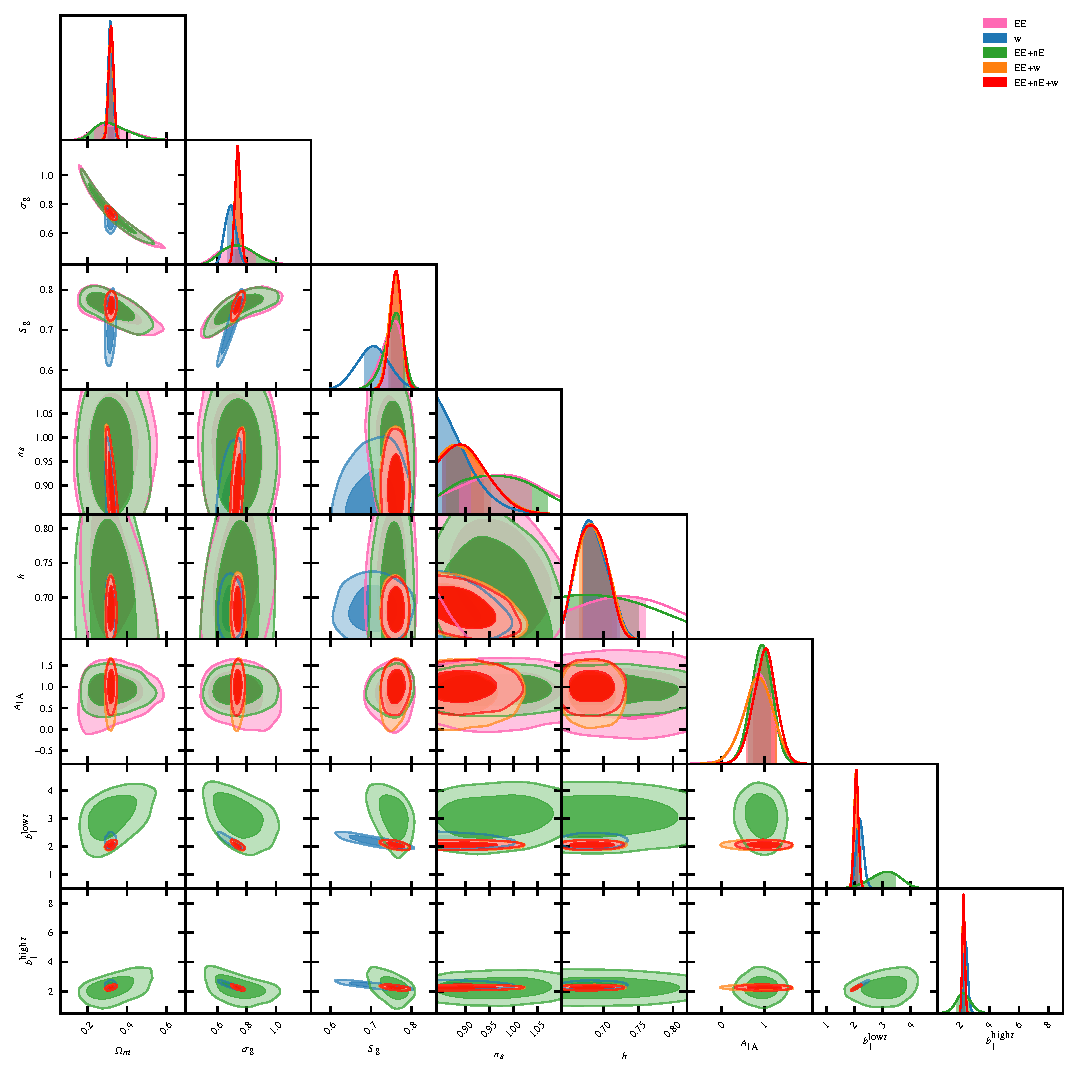
\includegraphics[width=\textwidth]{Parameter_Plots/omegam_sigma8_s8_ns_h_a_ia_b1l_b1h_blind_C}
		\caption{Constraints blind C}
		\label{fig:cosmology-params}
	\end{center}
\end{figure*}

\begin{table}
	\begin{center}
		\caption{Goodness of fit for blind A}
		\label{tab:goodness-of-fit}
\begin{tabular}{lrcl}
    \toprule
    Probe             & $\chi^2$       & DoF       & $p$-value   \\
    \midrule
	EE               & $< 156.3$ & $120-4.5$ & 0.007 \\
	w                & $< 176.0$ & $168-13$ & 0.119 \\
	EE+nE            & $< 187.7$ & $142-18$ & 0.000 \\
	EE+w             & $< 327.2$ & $288-20$ & 0.008 \\
	EE+nE+w          & $371.3$ & $310-20$ & 0.001 \\

    \bottomrule
\end{tabular}
	\end{center}
\end{table}

\begin{table}
	\begin{center}
		\caption{Goodness of fit for blind B}
		\label{tab:goodness-of-fit}
\begin{tabular}{lrcl}
    \toprule
    Probe             & $\chi^2$       & DoF       & $p$-value   \\
    \midrule
	EE               & $< 151.3$ & $120-4.5$ & 0.014 \\
	w                & $< 176.0$ & $168-13$ & 0.119 \\
	EE+nE            & $< 176.1$ & $142-18$ & 0.001 \\
	EE+w             & $< 328.0$ & $288-20$ & 0.007 \\
	EE+nE+w          & $351.3$ & $310-20$ & 0.008 \\

    \bottomrule
\end{tabular}
	\end{center}
\end{table}

\begin{table}
	\begin{center}
		\caption{Goodness of fit for blind C}
		\label{tab:goodness-of-fit}
\begin{tabular}{lrcl}
    \toprule
    Probe             & $\chi^2$       & DoF       & $p$-value   \\
    \midrule
	EE               & $< 150.8$ & $120-4.5$ & 0.015 \\
	w                & $< 176.0$ & $168-13$ & 0.119 \\
	EE+nE            & $< 178.5$ & $142-18$ & 0.001 \\
	EE+w             & $< 321.7$ & $288-20$ & 0.014 \\
	EE+nE+w          & $356.1$ & $310-20$ & 0.005 \\

    \bottomrule
\end{tabular}
	\end{center}
\end{table}
